\chapter{Wstęp}

Świat jest odwzorowywany przez programy komputerowe za pomocą modeli.
Zawierają one uproszczoną reprezentację rzeczywistości, a logika programu
umożliwia wykonywanie obliczeń na podstawie modelu, jego modyfikację, lub
utrwalenie i udostępnienie do wglądu innym osobom.
Modele te mogą być prezentowane użytkownikowi na wiele sposobów. Jednym z nich
jest reprezentacja graficzna w~formie diagramu. Taka metoda reprezentacji
ozwala użytkownikowi na łatwiejsze zrozumienie modelu
oraz jego modyfikację, w porównaniu do~formatu tekstowego, ponieważ jest
wizualna i przestrzenna, a więc jest naturalniejszą formą dla mózgu człowieka.

Przykładem modeli z reprezentacją graficzną, które są zrozumiałe zarówno dla
człowieka, jak i maszyny, oraz
przydają się podczas wytwarzania oprogramowania, są modele korzystające
z~\gls{UML}~\cite{wikipedia-uml}. Przedstawiają
one strukturę klas w programie oraz zależności między klasami. Na ich podstawie
czytelnik może wysokopoziomowo zapoznać się~ze strukturą programu, a
odpowiednie narzędzia pozwolą wygenerować kod klas w danym języku
programowania, który może służyć jako początek do późniejszego rozwoju
aplikacji. Przykładowy model \gls{UML} został przedstawiony na
rysunku~\ref{rys:przykladowy-model-uml}.

\begin{figure}[!hb]
	\centering
	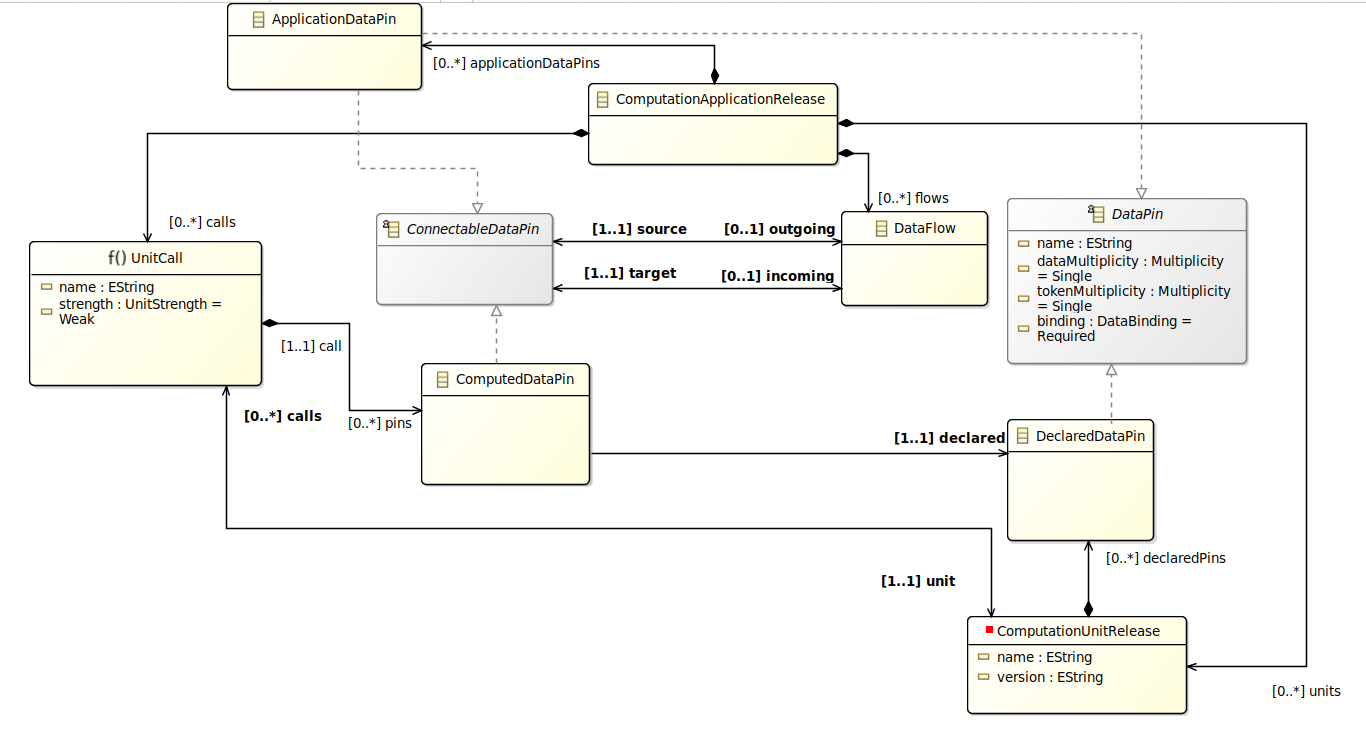
\includegraphics[width=0.95\linewidth]{./images/example-uml-model.png}
	\caption{Przykładowy model \gls{UML}.}\label{rys:przykladowy-model-uml}
\end{figure}

\gls{UML} jest przykładem uniwersalnego języka do opisu modeli klas programu.
Nie jest on~związany z żadną konkretną tematyką klas i pozwala na modelowanie
programów o~różnym zastosowaniu i przeznaczeniu. Istnieją także języki do opisu
modeli ściślej związanych z~konkretną dziedziną, czyli \gls{DSL}. Takie języki
są zazwyczaj mniejsze i mniej skomplikowane od języków uniwersalnych, a także
mają dokładniejszą semantykę (znaczenie elementów modelu). Potrafią więc one
odwzorować rzeczywistość w~sposób bardziej kompletny i zawrzeć więcej
szczegółów.

Strukturę samego modelu opisuje metamodel. Jest to model, który definiuje jakie
są~możliwe typy elementów modelu, jakie mają atrybuty, jak są połączone ze
sobą (składnia języka modelowania). Sam metamodel może być opisany na przykład
w języku UML\@ lub podobnym
bazowanym na nim, który będzie możliwiał wprowadzenie większej liczby
szczegółów. Taki metamodel często należy uzupełnić o zasady semantyczne ---
informacje o znaczeniu elementów, które nie mogą być zapisane w strukturze
metamodelu. Przykładową informacją semantyczną w modelu UML może być informacja
o krotności asocjacji.

\emph{BalticLSC} jest platformą do obliczeń rozproszonych wykonywaną z
inicjatywy
\emph{INTERREG Regionu Morza Bałtyckiego Unit Europejskiej}. Platforma ta
pozwala
wykonać obliczenia wykorzystując dostępne moduły obliczeniowe. Aplikacje
obliczeniowe definiowane są w postaci diagramów przedstawiających przepływ
danych między modułami obliczeniowymi. Przykład diagramu opisującego aplikację
obliczeniową został przedstawiony na
rysunku~\ref{rys:przykladowy-diagram-balticlsc}.  Model obliczeń opisany jest w
języku \gls{CAL}, który jest opisany za pomocą metamodelu~\cite{cal-metamodel}.

\begin{figure}[!hb]
	\centering

	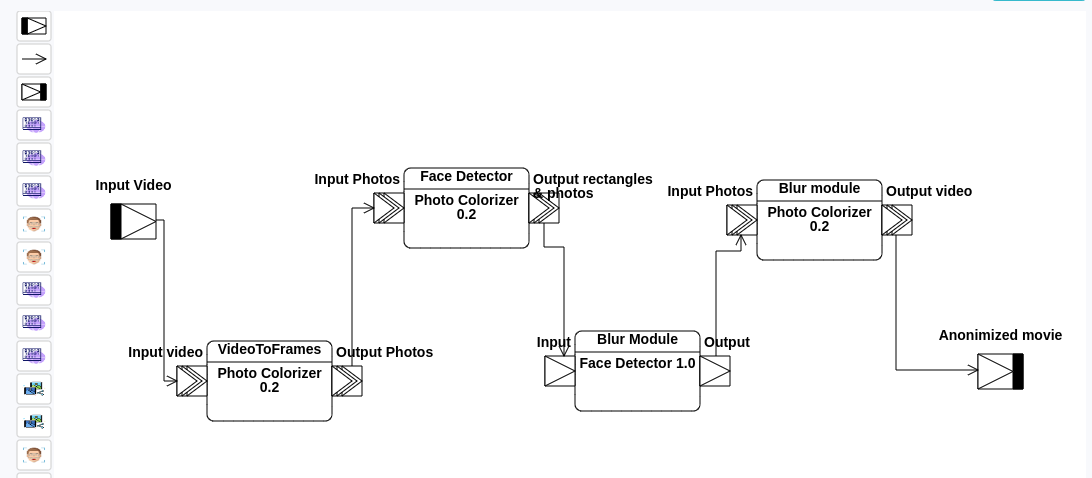
\includegraphics[width=0.95\linewidth]{./images/balticlsc-example-diagram.png}
	\caption{Przykładowy diagram przedstawiający aplikację obliczeniową w
		BalticLSC\@.}\label{rys:przykladowy-diagram-balticlsc}
\end{figure}

Istniejący edytor diagramów w BalticLSC dostępny jest jako część aplikacji
przeglądarkowej udostępnionej przez platformę. Do komunikacji z aplikacją
serwerową wykorzystuje inną reprezentację aplikacji obliczeniowej --- zapisuje
ją w postaci pudełek (prostokątów) oraz połączeń między nimi. Nie komunikuje
się on z aplikacją serwerową przesyłając informacje o strukturze modelu
zgodnej z metamodelem języka \gls{CAL}. Sprawia to, że po obu stronach (serwera
i aplikacji przeglądarkowej) potrzebne są dodatkowe transformacje
przetwarzające ogólny opis diagramu na model aplikacji obliczeniowej.

Sirius Web~\cite{sirius-web-github} jest narzędziem przygotowywanym przez firmę
Eclipse do tworzenia edytorów
diagramów działających w przeglądarce bazujących na metamodelach \gls{EMF}.
Technologia \gls{EMF} jest wykorzystywana od roku
2007~\cite{eclipse-sirius-wikipedia}, a metamodele
w~przeszłości mogły być tworzone używając oprogramowania Sirius
Desktop. Wykorzystując Sirius Web można w prosty sposób otrzymać aplikację
przeglądarkową umożliwiającą możliwości przeglądania i edycji modeli zbliżone
do tych,
które dotychczas oferowała jedynie aplikacja wymagająca instalacji na
komputerze użytkownika. Oprócz łatwiejszego dostępu do edytora diagramów dla
nowych użytkowników, wykorzystanie technologii przeglądarkowych do budowy
edytora diagramów pozwalają na dodanie mechanizmów kontroli dostępu do
wybranych modeli dla pewnych użytkowników, a także możliwości współpracy nad
modelem przez różne osoby w~czasie rzeczywistym.

W ustrukturyzowanym modelu zawierającym obiekty dziedzinowe w nietrudny sposób
można wyrazić reguły determinujące poprawność semantyczną modelu. Sirius
Desktop pozwala w tym zakresie na definiowanie semantycznych reguł
walidacyjnych, które są uruchamiane po każdej modyfikacji modelu i pokazują
błędnie umieszczone elementy. Odpowiednik tej funkcjonalności jest pożądany
także w edytorach diagramów opartych na Sirius Web.

W ramach tej pracy magisterskiej przygotowany został edytor diagramów dla
systemu BalticLSC korzystający z \emph{Sirius Web}. Edytor ten bazuje na
formalnym metamodelu \gls{EMF} opisującym język \gls{CAL} do
opisu aplikacji obliczeniowej. Ponadto, dostarczona została metoda sprawdzania
poprawności przygotowywanych przez użytkownika modeli na podstawie
zdefiniowanych reguł walidacji.

\section{Motywacja i cel pracy}

Jedną z alternatyw do wykorzystania Sirius Web do budowy edytora diagramów jest
wykorzystanie gotowych bibliotek JavaScript do wyświetlania i modyfikacji
diagramów (przykłady: \emph{react-diagrams}~\cite{react-diagrams-github},
\emph{Cytoscape.js}~\cite{cytoscape-js-homepage},
\emph{vis-network}~\cite{vis-network-github}). Są one ogólnymi narzędziami
pozwalającymi na zbudowanie własnego edytora diagramów. Dają sporą dowolność w
kwestii wyświetlania diagramu oraz
dostępnych funkcjonalności. Nie narzucają one
wykorzystania ustrukturyzowanych modeli poprzez wymaganie stworzenia
metamodelu. Z uwagi na swoją ogólność są trudniejsze do dostosowania do
własnych potrzeb, ponieważ funkcjonalności takie jak zapisywanie modeli w bazie
danych, współpraca w czasie rzeczywistym, walidacja modelu należy
zaimplementować samemu. Ponadto, modyfikacja takiego edytora diagramów wymaga
znajomości języka JavaScript.

Sirius Web dostarcza większość z tych
funkcjonalności wymagając jedynie wskazania metamodelu, który ma wykorzystywać.
Korzyści płynące z łatwego do przygotowania przeglądarkowego edytora diagramów
dla wybranych przez
nas modeli prezentują technologię Sirius Web jako interesującą i wartą użycia,
pomimo jej wczesnej fazy rozwoju i braku dokumentacji.

Celem tej pracy magisterskiej jest zbadanie możliwości udostępnianych przez
Sirius Web poprzez wykorzystanie go do przygotowania edytora
diagramów dla modeli języka CAL na platformie BalticLSC\@. Elementem edytora,
na który należy zwrócić szczególną uwagę, jest możliwosć walidacji modeli,
czyli weryfikacji ich~poprawności strukturalnej i semantycznej.

Ponadto, praca ta będzie jednym z pierwszych zastosowań Sirius Web wykonanych
przez osoby spoza zespołu budującego tą technologię, co może dostarczyć
dodatkowych informacji zwrotnych na temat prostoty jego wykorzystania, a także
napotkanych błędów i~niedociągnięć. Dla osób rozważających budowę edytora
modeli w oparciu o Sirius Web, praca ta będzie stanowiła źródło informacji o
wrażeniach z wykorzystania tej technologii, co pomoże podjąć bardziej świadomą
decyzję o używanych technologiach.
Z uwagi na brak dostępnej dokumentacji Sirius Web, praca ta może służyć również
jako przykład wykorzystania własnego metamodelu w tym edytorze diagramów.

Taki edytor diagramów bazujący na Sirius Web mógłby również zostać wykorzystany
w~aplikacji przeglądarkowej platformy BalticLSC\@. Jest on oparty o
ustrukturyzowany opis modelu, co pozwoliłoby na uproszczenie metody komunikacji
między serwerem aplikacyjnym a~aplikacją przeglądarkową, ponieważ nie byłyby
wymagane transformacje z aktualnego, ogólnego formatu danych do formatu
zgodnego z metamodelem.

\section{Zakres pracy}

W ramach pracy magisterskiej wykonano następujące czynności:

\begin{itemize}
	\item Stworzenie metamodelu języka \gls{CAL} w \gls{EMF}\@ z wykorzystaniem Sirius Desktop.
	\item Wykorzystanie tego metamodelu w Sirius Web. Zgłoszenie usterek autorom Sirius Web poprzez GitHub.
	\item Porównanie możliwości Sirius Web i Sirius Desktop. Zgłoszenie brakujących funkcjonalności autorom Sirius Web poprzez GitHub.
	\item Dodanie do metamodelu elementów usprawniających pracę z nim (automatyzacja niektórych czynności, dodanie ograniczeń utrudniających zrobienie błędu).
	\item Modyfikacja przeglądarkowego interfejsu użytkownika Sirius Web poprzez dodanie do niego przybornika z BalticLSC\@. Przybornik umożliwia w łatwy sposób dodanie nowych elementów do modelu.
	\item Dodanie mechanizmu walidacji semantycznej modelu sprawdzającego poprawność modelu z regułami zdefiniowanymi w języku Java.
	\item Stworzenie planu integracji rozwiązania z BalticLSC\@.
	\item Stworzenie przykładowej aplikacji przeglądarkowej zawierającej jedynie edytor diagramów z Sirius Web. Taki przykład pokazuje możliwość wykorzystania Sirius Web jako element innej aplikacji przeglądarkowej.
\end{itemize}

\vspace{1em}

\noindent Poza zakresem pracy pozostały następujące czynności:

\begin{itemize}
	\item Integracja stworzonego rozwiązania jako alternatywnego edytora diagramów dla systemu BalticLSC\@.
	\item Naprawa zgłoszonych usterek w Sirius Web.
\end{itemize}

\chapter{Tworzenie edytorów graficznych na bazie metamodeli}

Aplikacje komputerowe wykorzystują elementy graficzne aby ułatwić i
przyśpieszyć użytkownikom pracę.
Dzieje się to z uwagi na fakt, że ludzie bardziej efektywnie przyswajają
informacje wizualne (obrazki, diagramy), niż
tekst~\cite{images-more-effective-article}.
W przypadku użytkownika
wpływającego na~zachowanie systemu w sposób wizualny (np.\ edytując diagram),
korzysta on wtedy z~edytora graficznego i modyfikuje pewien model
rzeczywistości reprezentowany przez program. Model ten zaprojektowany jest
przez twórcę aplikacji i jego struktura również może być~reprezentowana na
wiele sposobów. Jeżeli struktura modelu sama jest opisywana przez model (o
wyższym poziomie abstrakcji) to mówimy, że~ten model modelu to
\emph{metamodel}.

\section{Metamodelowanie}

\emph{Metamodelowanie} w kontekście wytwarzania oprogramowania to
technika polegająca
na~przygotowaniu abstrakcyjnego modelu (metamodelu) opisującego strukturę
modeli, które będą wykorzystywane w programie. Metamodel określa jakie są
dopuszczalne typy obiektów w~modelu, ich atrybuty, powiązania między nimi.
Definiuje składnię języka projektowania. Przedrostek \emph{meta} oznacza, że
poziom abstrakcji tego metamodelu jest wyższy niż poziom abstrakcji modelu,
który opisuje~\cite{from-requirements-to-java-in-a-snap}.

W rodzinie metamodeli przestrzenią o najmniejszym poziomie abstrakcji jest
świat rzeczywisty (przestrzeń \emph{M0}). W programach komputerowych będzie on
reprezentowany przez model, który znajduje się w przestrzeni o wyższym poziomie
abstrakcji, \emph{M1}. Idąc dalej, modele będą oparte na metamodelach dla danej
dziedziny, które znajdują się w przestrzeni \emph{M2}. One~z~kolei są oparte na
meta--metamodelach % chktex 8
z przestrzeni \emph{M3}, które mają najwyższy poziom
abstrakcji w tej rodzinie. \emphgls{MOF}~\cite{mof-omg-specification} jest
przykładem meta--metamodelu. % chktex 8
Jest~zdefiniowany za pomocą samego siebie.

% TODO: dodać referencję z bibliografii

Wiele powszechnie znanych języków projektowania diagramów ma swoje metamodele
definiujące ich strukturę:

\begin{itemize}
	\item \emphgls{UML} ma swoją specyfikację~\cite{uml-omg-specification}
	      i metamodel opisany w języku \emphgls{MOF}.

	\item \emphgls{BPMN} (język do opisu procesów biznesowych) ma swój
	      metamodel~\cite{bpmn-omg-specification} również opisany w języku \emphgls{MOF}.

	\item Istnieje artykuł proponujący metamodel dla \emphgls{ERM}~\cite{entity-relationship-metamodel}. Dla~przypomnienia, \emphgls{ERM} pozwala przedstawić na diagramie encje bazy danych i~powiązania między nimi.
\end{itemize}

W metamodelu zdefiniowana jest składnia abstrakcyjna modelu, czyli struktura
jego elementów, oraz składnia konkretna, czyli jak one mają być reprezentowane,
na przykład na~diagramie.
Aby model był funkcjonalny oprócz jego struktury (składni języka projektowania)
należy zdefiniować i przestrzegać jego semantyki. To ona decyduje o tym jak
należy interpretować model, a także jakie sytuacje, pomimo bycia poprawnymi
strukturalnie, byłyby niewłaściwe z~punktu widzenia ich sensowności.

Przykładowo, w języku \emphgls{UML} z perspektywy struktury możliwe jest
utworzenie dwóch klas i dwóch połączeń kompozycji między nimi, co zostało
zademonstrowane na rysunku~\ref{rys:nieprawidlowy-model-uml}. Taki model jest
semantycznie niepoprawny, ponieważ relacja kompozycji oznacza, że jeden obiekt
jest zawarty w drugim obiekcie. Oznaczałoby to, że zarówno osoba
(\emph{Person}) jest zawarta w obiekcie samochodu (\emph{Car}) jako jego
właściciel, jak i samochody są zawarte w obiekcie właściciela.

\begin{figure}[!hb]
	\centering

	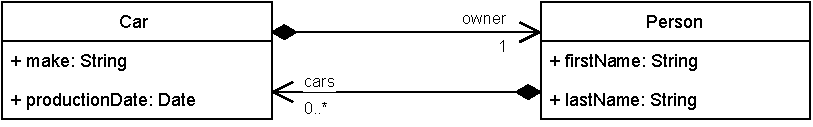
\includegraphics[width=0.95\linewidth]{./images/invalid-uml-example.pdf}
	\caption{Przykład modelu \emphgls{UML} nieprawidłowego
		semantycznie}\label{rys:nieprawidlowy-model-uml}
\end{figure}

Dopiero znając znaczenie relacji kompozycji można zauważyć ten błąd semantyczny
i~go~poprawić, na przykład jak na rysunku~\ref{rys:prawidlowy-model-uml}. Na
tym diagramie to osoba (\emph{Person}) jest obiektem nadrzędnym, który może
zawierać w sobie odniesienia do samochodów (\emph{Car}). Taki diagram jest
poprawny zarówno składniowo, jak i semantycznie.

\begin{figure}[!hb]
	\centering

	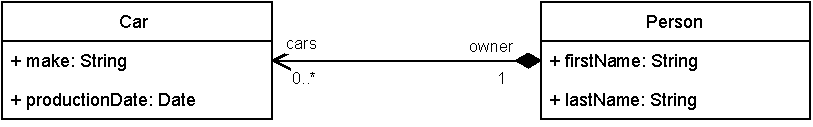
\includegraphics[width=0.95\linewidth]{./images/valid-uml-example.pdf}
	\caption{Przykład prawidłowego modelu
		\emphgls{UML}}\label{rys:prawidlowy-model-uml}
\end{figure}

\section{Edytory graficzne na podstawie metamodeli}

Metamodele mogą być zapisane w formacie, który jest przyjazny do odczytu
maszynowego. Oznacza to, że narzędzia będą mogły go odczytać, zinterpretować, a
także edytować. Sam~metamodel może mieć swój meta-metamodel, który zdefiniuje
jego strukturę.

Taki sformalizowany sposób przechowywania metamodelu ma wiele
korzyści. Przede wszystkim metamodel może być wtedy projektowany i edytowany w
narzędziu umożliwiającym robienie tego w najprostszy dla użytkownika sposób, na
przykład poprzez reprezentację metamodelu jako diagram. Ponadto, narzędzia mogą
wygenerować kod w konkretnym języku programowania. Zawierać on może klasy lub
inne mechanizmy przedstawienia modelu w tym języku programowania oraz może
wspierać operacje takie jak edycja, sprawdzenie poprawności składniowej
modelu.

Skoro znana jest struktura modelu, a więc wszystkie możliwe elementy i ich
połączenia, możliwe jest stworzenie edytora modeli, który będzie oparty na
metamodelu. Otrzymanie edytora diagramów dla danej dziedziny odbywa się dzięki
temu niskim nakładem czasowym --- wystarczy zdefiniować metamodel dziedziny, a
także zdefiniować wygląd elementów. Wymaga to mniejszej ilości czasu i
umiejętności w porównaniu z budową edytora diagramów korzystając z
edytorów diagramów ogólnego zastosowania.

\begin{figure}[!b]
	\centering

	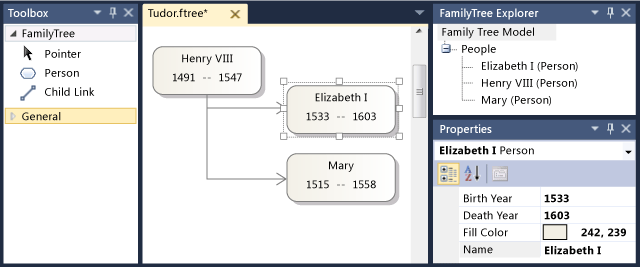
\includegraphics[width=0.95\linewidth]{./images/visual-studio-dsl-example.png}
	\caption{Edytowanie modelu w \emph{Visual Studio DSL
			Tools}}\label{rys:visual-studio-dsl-example}
\end{figure}

Przykładem zestawu narzędzi dostarczającego możliwości metamodelowania i
późniejszego generowania edytora graficznego dla modelu jest \emph{Visual
	Studio DSL Tools}~\cite{visual-studio-dsl-introduction} utworzone przez
firmę \emph{Microsoft}. Jest to zestaw
narzędzi do definiowania metamodelu, a następnie przygotowania rozszerzenia do
\emph{Visual Studio} w formacie \emphgls{VSIX}. Po jego zainstalowaniu
\emph{Visual Studio} nabiera możliwości graficznego edytowania modeli
bazujących na danym metamodelu. Edycja przykładowego modelu przedstawiona jest
na rysunku~\ref{rys:visual-studio-dsl-example}. Ponadto, tak przygotowany
edytor
może również generować klasy języka \emph{C\#} pozwalające na reprezentację
modelu, a
także jego serializację i deserializację. Dodatkową funkcjonalnością jest
również możliwość tworzenia plików na podstawie szablonów przygotowanych dla
metamodelu. W ten sposób można wygenerować na przykład tabelę w~języku
\emphgls{HTML} zawierającą wszystkie elementy konkretnego typu w modelu.

Innym narzędziem umożliwiającym przygotowanie edytora graficznego na podstawie
metamodelu jest \SiriusDesktop{}~\cite{sirius-desktop-homepage} rozwijany
przez firmę \Eclipse{}. Jest to rozszerzenie do~zintegrowanego środowiska
programistycznego (\emphgls{IDE}) \Eclipse{}. Pozwala ono na zaprojektowanie
metamodelu dla wybranej dziedziny używając technologii \emph{\acrfull{EMF}}.
Jest on wyrażony za pomocą
meta--metamodelu  % chktex 8
\Ecore{} (rozszerzenie \texttt{*.ecore}) i jest
zapisany w pliku \emphgls{XML}. Interfejs użytkownika programu \SiriusDesktop{}
widoczny jest na rysunku~\ref{rys:sirius-desktop-example-metamodel}. Po lewej
dostępne jest drzewo metaklas, na środku widać diagram struktury struktury
metamodelu, a po prawej stronie znajduje się przybornik z~narzędziami do
tworzenia elementów metamodelu. W \SiriusDesktop{}
można wygenerować 5 pakietów opisanych w kolejnych akapitach.

\begin{figure}[!ht]
	\centering

	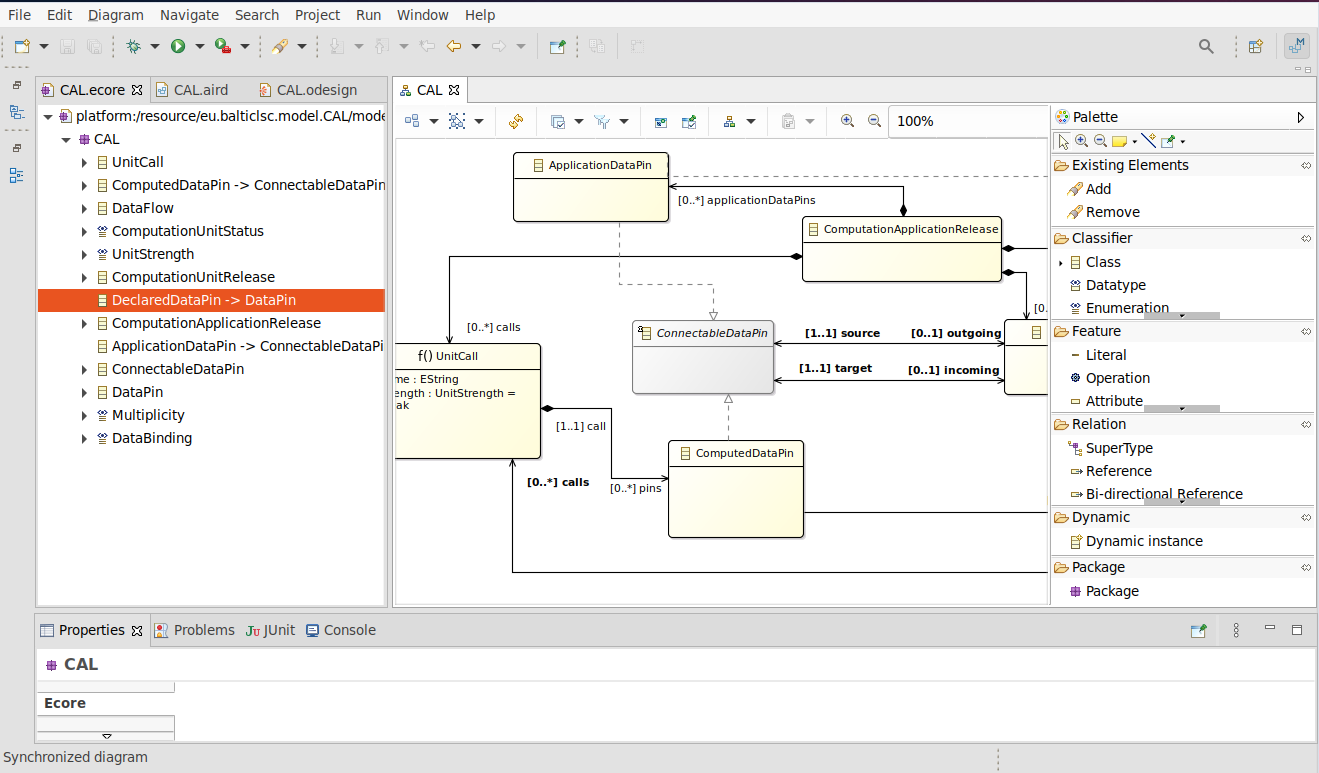
\includegraphics[width=0.95\linewidth]{./images/sirius-desktop-metamodel.png}
	\caption{Projektowanie metamodelu w \emph{Sirius
			Desktop}}\label{rys:sirius-desktop-example-metamodel}
\end{figure}

Pierwszym pakietem jest pakiet bazowy zawierający klasy umożliwiające
reprezentację modeli w
kodzie języka \Java{}, ich serializację i deserializację. Każdy obiekt
metamodelu
odpowiada klasie języka \Java{}. Klasy te zawierają mechanizmy powiadamiana o
zmianach (ang.~\emph{\selectlanguage{english}change detection}).
Możliwa jest modyfikacja kodu tych klas, co zmienia zachowanie
modelu.

Drugim z pakietów jest pakiet \texttt{.design} z plikiem o rozszerzeniu
\texttt{*.odesign} zawierający opis reprezentacji graficznych modelu. Każdy
model może mieć wiele reprezentacji graficznych z~różnymi poziomami
szczegółowości.
Możliwe reprezentacje graficzne to diagram klas, diagram
sekwencji, tabela, drzewo~\cite{dokumentacja-sirius-desktop}. Dla każdej
reprezentacji należy zdefiniować jak elementy modelu mają być wyświetlane.

Funkcjonalności ulepszające doświadczenia użytkownika z
korzystania z edytora zawierają także możliwość ustalenia styli warunkowych
(zmiany wyglądu elementu gdy spełnione zostaną ustalone warunki), zdefiniowanie
narzędzi pomagających w edycji diagramu (przykładowo okno dialogowe
wyświetlające formularz składający się z kilku kroków, który ostatecznie tworzy
kilka powiązanych ze sobą obiektów w modelu, albo narzędzie do kaskadowego
usuwania powiązanych elementów modelu), jak i możliwość opisania reguł
walidacji semantycznej, które będą uruchamiane po każdej zmianie i będą mogły
oznaczyć niepoprawne elementy modelu oraz zaproponować automatyczne ich
naprawienie.

Operacje wymagające wykonania dynamicznej logiki mogą być wprowadzone na 2
sposoby: poprzez napisanie kodu w języku \Java{} i udostępnienie go jako usługa
dostępna w~metamodelu, lub poprzez napisanie wyrażenia w języku
\emphgls{AQL}~\cite{dokumentacja-aql}.
Pozwala on~na~wybranie elementów z modelu (także podzbioru elementów
spełniających pewne kryteria), ich~atrybutów, oraz wykonanie operacji
logicznych na nich, na przykład ich~porównanie.

Trzecim pakietem jest pakiet \texttt{.edit}. Składa się on z klas
umożliwiających programatyczne odczytanie informacji o strukturze modelu ---
klasy zawierają opis właściwości obiektów modelu.

Czwartym pakietem jest pakiet \texttt{.editor}. Zawiera on definicję wtyczki do
środowiska \Eclipse{}, która dostarcza możliwości tworzenia i edycji
modeli. To właśnie ten pakiet umożliwia użycie wszystkich pozostałych pakietów
przez użytkownika i ostatecznie otrzymanie edytora graficznego. Edytor
diagramów dla przykładowego modelu został zaprezentowany na
rysunku~\ref{rys:sirius-desktop-example-model}.

\begin{figure}[!ht]
	\centering

	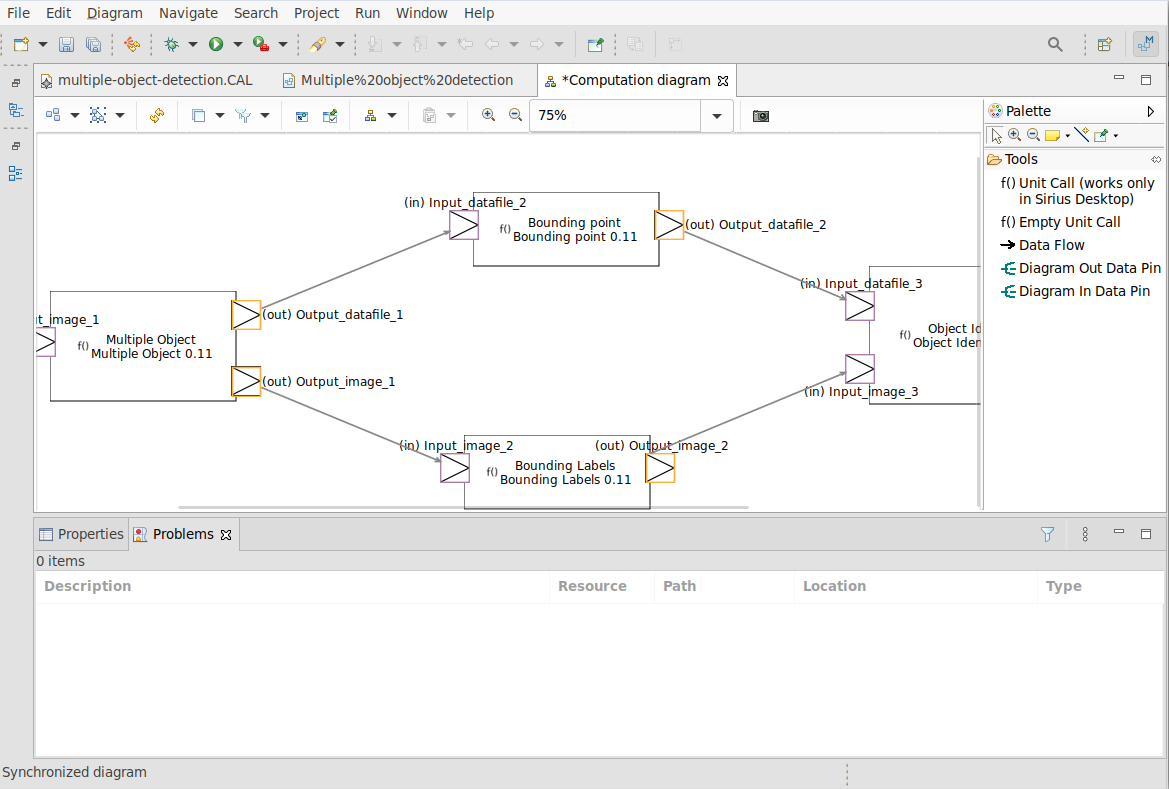
\includegraphics[width=0.95\linewidth]
	{./images/sirius-desktop-model-editor.png}
	\caption{Edycja przykładowego modelu w
		\SiriusDesktop{}}\label{rys:sirius-desktop-example-model}
\end{figure}

Piątym pakietem jest pakiet \texttt{.tests}. Można w nim tworzyć testy
zachowania metamodelu korzystając z środowiska uruchomieniowego do testów
\JUnit{}. Testy te przydają się~gdy~domyślne zachowanie modelu zostanie
zmodyfikowane poprzez edycję klas bazowych modelu w~głównym pakiecie projektu.

Edytor graficzny otrzymany dzięki pakietowi \texttt{.editor} jest wtyczką do
środowiska \Eclipse{}, które jest aplikacją systemową wymagającą instalacji
w systemie użytkownika zanim będzie on~mógł przeglądać i edytować modele.
Od 2018 roku~\cite{sirius-components-repo-first-commit} firma \Eclipse{}
pracuje nad~rozwiązaniem \SiriusWeb{}~\cite{sirius-web-github}, którego
celem jest przeniesienie edytora
graficznego dotychczas dostępnego w aplikacji natywnej do przeglądarki
internetowej. Interfejs użytkownika tego projektu jest widoczny na
rysunku~\ref{rys:sirius-web-ui}.

\begin{figure}[!ht]
	\centering

	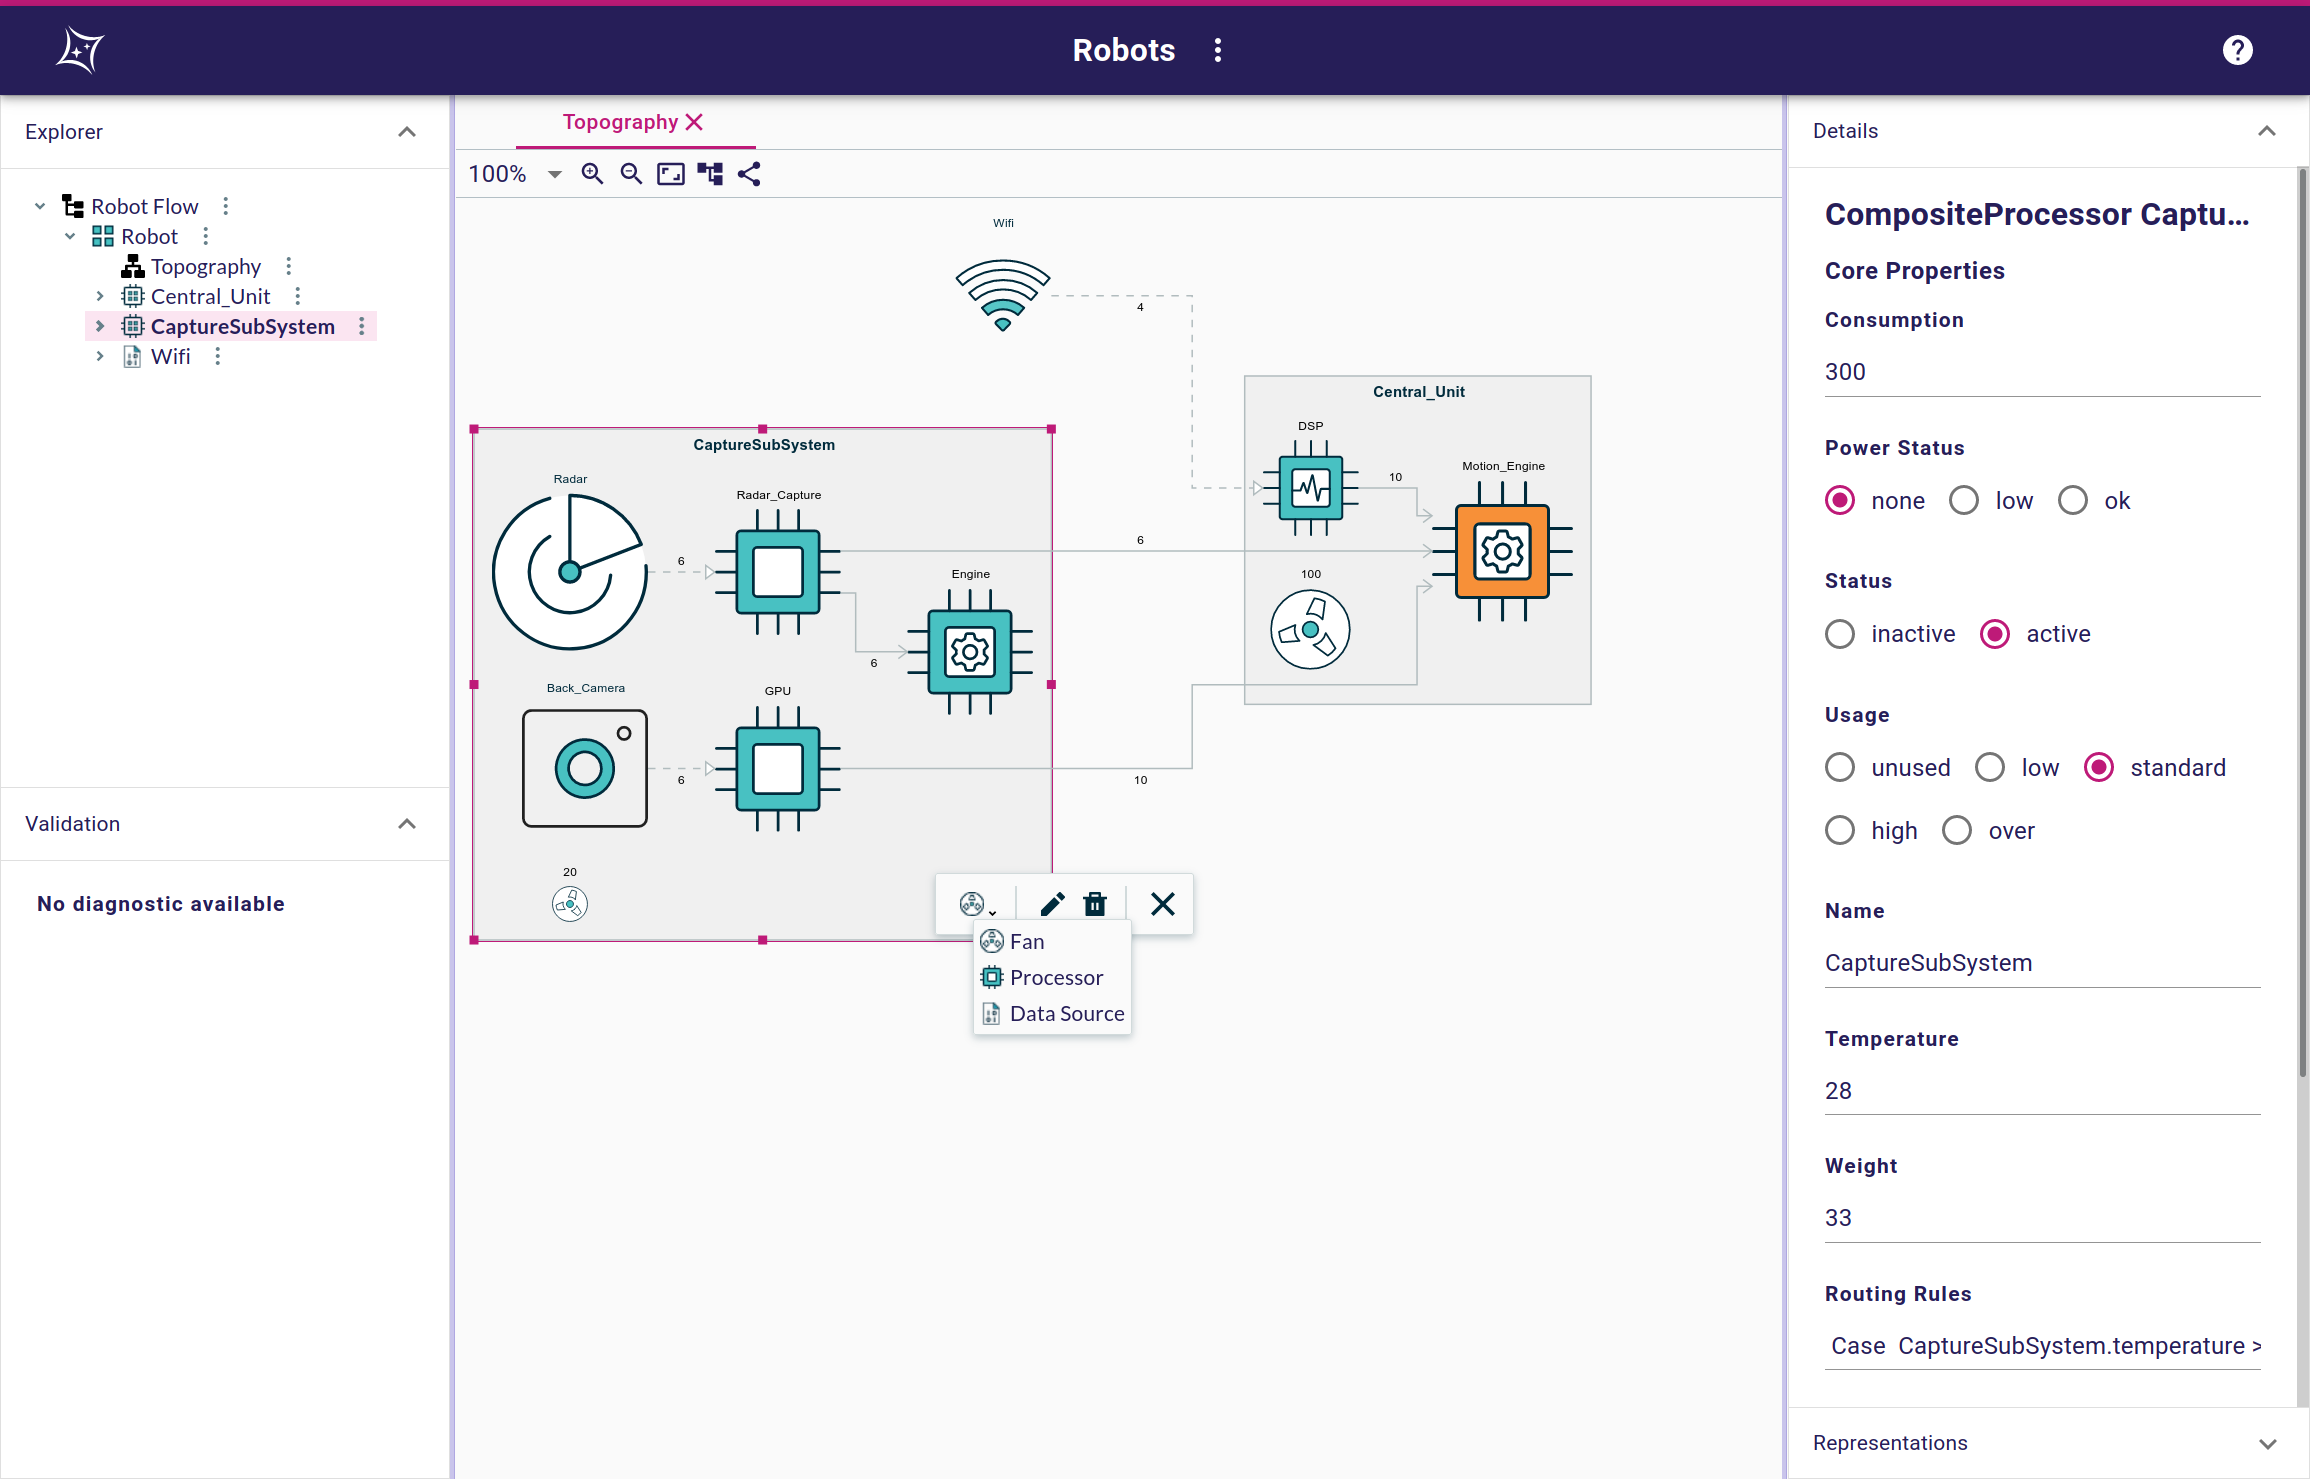
\includegraphics[width=0.95\linewidth]
	{./images/sirius-web-editor.png}
	\caption{Edytor modeli \SiriusWeb{}}\label{rys:sirius-web-ui}
	{\small Źródło: \url{https://github.com/eclipse-sirius/sirius-web}}
\end{figure}

\SiriusWeb{} składa się z 3 komponentów:

\begin{itemize}
	\item serwera aplikacyjnego stworzonego w technologii \emph{Java
		      Spring}~\cite{java-spring-homepage} dostarczającego interfejsu sieciowego \emphgls{API} w formacie \GraphQL{} pozwalającego na wyświetlenie oraz modyfikację modelu,
	\item bazy danych \PostgreSQL{}~\cite{postgresql-homepage} przechowującej informacje o modelach i użytkownikach,
	\item aplikacji przeglądarkowej napisanej z wykorzystaniem biblioteki \React{}~\cite{react-homepage} umożliwiającej wyświetlenie i modyfikację modeli w formie drzewa obiektów lub diagramu.
\end{itemize}

Metamodele, na których bazuje \SiriusWeb{} są w tym samym formacie \Ecore{} co
metamodele w \SiriusDesktop{}. Można zatem w łatwy sposób stworzyć
graficzny edytor modeli zarówno w~formie aplikacji natywnej, jak i
przeglądarkowej. Posiadając istniejący metamodel języka użyty
w~\SiriusDesktop{} można go w krótkim czasie przenieść do \SiriusWeb{}. Jest
to~możliwe, ponieważ serwer aplikacyjny korzysta z tych samych bibliotek i
pakietów do obsługi metamodelu, które są wykorzystywane w edytorze
\SiriusDesktop{}.

Zmianie uległ natomiast sposób przechowywania modeli. W \SiriusDesktop{}
były one~zapisane w plikach na dysku użytkownika. W \SiriusWeb{} są one
przechowywane w bazie danych \PostgreSQL{}. Taki format zapisu pozwala na
równoczesny dostęp do modelu przez wielu użytkowników i natychmiastowe
przesyłanie informacji o zmianach w czasie rzeczywistym dzięki użyciu
\emph{GraphQL Subscriptions}~\cite{graphql-subscriptions} (dwukierunkowych
połączeń do przesyłania ustrukturyzowanych danych między przeglądarką a
serwerem opartych na protokole \WebSocket{}~\cite{wikipedia-websocket}).
Oznacza to, że użytkownicy mogą w czasie rzeczywistym wspólnie edytować modele
i~natychmiast widzieć zmiany wprowadzone przez innych użytkowników.
Poprzez zgrupowanie modeli w~projekty wewnątrz aplikacji \SiriusWeb{}
możliwa jest również kontrola dostępu do nich --- administrator może określić
zasady dostępu użytkowników do poszczególnych projektów.

Udostępnienie edytora modeli jako aplikacja przeglądarkowa sprawia też, że jest
on~bardziej dostępny dla użytkowników. Mogą oni przeglądać i edytować modele
bez instalacji aplikacji natywnych w ich systemie --- wystarczy przeglądarka
internetowa, która jest zainstalowana na większości komputerów konsumenckich.
Można też w łatwiejszy sposób podzielić się~przygotowanym przez nas modelem,
ponieważ wystarczy wysłać adres \emphgls{URL} innemu użytkownikowi zamiast
wysyłać plik z modelem.

Poza tym łatwiejsze wprowadzanie jest poprawek i zmian do metamodelu.
W przypadku aplikacji natywnych i dzieleniu się modelem przechowywanym w pliku
należało zaktualizować metamodel oraz wszystkie jego modele, a później wysłać
nowe pliki modeli oraz nowy edytor wszystkim użytkownikom. Problemy powstają
gdy użytkownicy zmodyfikowali swoje modele przechowywane lokalnie i nie są już
one kompatybilne z nowym metamodelem, lub gdy użytkownicy przypadkowo używają
starego modelu przy pracy z modelami. Takie rozwiązanie zwiększa liczbę
możliwości na popełnienie błędu. W przypadku aplikacji internetowej wszyscy
pracują z~tymi samymi modelami przechowywanymi na serwerze. Osoby
odpowiedzialne za~metamodel mogą go zmodyfikować wraz z modelami zapisanymi w
bazie danych. Uruchomienie serwera z~nowym metamodelem wystarcza, aby wszyscy
użytkownicy po~otworzeniu edytora \SiriusWeb{} mieli jego najnowszą
wersję.


\chapter{Metamodel dla języka CAL}

W tym rozdziale zostanie omówione przygotowane rozwiązanie.

\section{Język opisu obliczeń w BalticLSC}

\section{Stworzony metamodel EMF dla języka CAL}

Omówienie przygotowanego modelu. Zrzut ekranu przedstawiający model. Omówienie
elementów oraz jakie one mają przełożenie na wykonanie obliczeń przez
BalticLSC\@.

\subsection{Warunkowa zmiana stylu elementów}

Omówienie reguł warunkowej zmiany stylu elementów diagramu:

\begin{enumerate}
	\item \texttt{DataPin} zmieniają ikonę na podstawie swoich \textit{data
		      multiplicity} oraz \textit{token multiplicity}.
	\item \texttt{ComputedDataPin} zmieniają kolor na podstawie swojego
	      \textit{data binding}.
\end{enumerate}

\subsection{Narzędzia edytora diagramów}

Omówienie dodanych \textit{Tools} z Sirius:

\begin{itemize}
	\item usunięcie \texttt{UnitCall} lub \texttt{ApplicationDataPin} usuwa również powiązane \texttt{DataFlow}
	\item usunięcie \texttt{ComputedDataPin} z poziomu edytora diagramów nie jest możliwe
	\item ograniczenia na tworzenie \texttt{DataFlow} tak, aby były semantycznie poprawne
	\item automatyczne usuwanie i tworzenie \texttt{ComputedDataPin} po zmianie \texttt{ComputationUnitRelease} dla danego \texttt{UnitCall}
	\item okno dialogowe ułatwiające tworzenie \texttt{UnitCall} dla istniejącego \texttt{ComputationUnitRelease}
	\item \ldots
\end{itemize}

\subsection{Reguły walidacyjne powiązane z
	metamodelem}\label{sec:regulky-walidacyjne-metamodel}

Omówienie \textit{semantic validation rule} z pliku \texttt{*.odesign}, które
działają w Sirius Desktop.

\subsection{Testy metamodelu}

Omówienie dodanych testów jednostkowych modelu (głównie dotyczy automatycznego
zarządzania \texttt{ComputedDataPin} w zależnosci od
\texttt{ComputationUnitRelease} dla konkretnego \texttt{UnitCall}).

\chapter{Dostosowanie Sirius Web dla systemu BalticLSC}

\section{Użycie metamodelu języka CAL w Sirius Web}

Opis jak wykorzystać metamodel EMF w Sirius Web.

\begin{itemize}
	\item konfiguracja Maven
	\item odpowiednia modyfikacja klas Javy w Sirius Web
\end{itemize}

\noindent oraz jaki rezultat uzyskano.

\section{Integracja przybornika BalticLSC w Sirius Web}

Opis problemu dodawania nowych \texttt{UnitCall} do diagramu --- trzeba
zdefiniować \texttt{ComputationUnitRelease} w diagramie.

Rozwiązanie (zaczerpnięte z edytora diagramów BalticLSC) --- przybornik
(toolbox).

Opis jak to zrobiono, od strony backendu jak i frontendu. Omówienie trudności w
modyfikacji interfejsu użytkownika Sirius Web (trzeba było skopiować kod
źródłowy niektórych komponentów z biblioteki \textit{Sirius Components} do kodu
aplikacji Sirius Web, ponieważ komponenty te nie umożliwiały modyfikacji
interfejsu i wstawiania do nich nowych elementów --- najlepiej dać zrzut ekranu
co można było łatwo zmienić, a co wymagało skopiowania kodu).

\section{Walidacja semantyczna modelu}

Informacja o informacjach diagnostycznych udostępnianych domyślnie przez Sirius
Web.

Brak uruchamiania reguł semantycznych zdefiniowanych w
metamodelu~\ref{sec:regulky-walidacyjne-metamodel}.

Opis dodanego rozwiązania (własne klasy Javowe które zwracają listę informacji
diagnostycznych, oraz strumieniowanie ich do przeglądarki wykorzystując
istniejące rozwiązanie do walidacji).

\section{Użycie edytora Sirius Web w BalticLSC}

Omówienie przygotowanego planu integracji.

\chapter{Ocena Sirius Web}

\section{Różnice między Sirius Web a Sirius Desktop}

Omówienie różnic oraz usterek zgłoszonych przeze mnie w repozytorium Sirius
Web.

\section{Użycie własnego metamodelu}

\section{Dodawanie funkcjonalności do edytora}

\chapter{Informacje techniczne}

\section{Wykorzystane biblioteki}

Tabela z wykorzystywanymi bibliotekami i ich licencjami.

\section{Projekt systemu}

Diagram z backendami oraz frontendami BalticLSC, a także bazą danych
PostgreSQL\@.

\section{Projekt modułów}

Informacje o modułach backendu (projekty Javy w Sirius Web).

\section{Instrukcja wdrożenia}

\subsection{Wymagania}

Docker, lub Java 11, Maven, PostgreSQL

\subsection{Instrukcja instalacji}

Opis: albo Docker, albo instalacja manualna (potwórzenie instrukcji z
\texttt{README.md}).

\subsection{Instrukcja uruchomienia}

Opis: albo Docker, albo manualnie uruchomienie serwera

\section{Instrukcja użycia}

Jak użyć aplikacji do stworzenia prostego modelu

Powinno także zawierać informacje o logowaniu się do BalticLSC\@.

\section{Instrukcja utrzymania}

\subsection{Kopia zapasowa bazy danych}

Jak stworzyć kopię bazy w PostgreSQL\@?

\subsection{Aktualizowanie wersji Sirius Web}

Opis metody aplikowania najnowszych zmian z repozytorium Sirius Web
(generowanie \texttt{git patch} i aplikowanie ich).

\section{Zabezpieczenia}

Brak zabezpieczeń.

\section{Testy akceptacyjne rozwiązania}

Opis kilku testów, które użytkownik może chcieć wykonać aby sprawdzić, czy
rozwiązanie działa poprawnie.

\subsection{Wynik testów akceptacyjnych}

Czy się udały?

\chapter{Podsumowanie}

\section{Wyniki pracy}

Co zostało osiągnięte? Czy cel został zdobyty?

\section{Wnioski}

Sirius Web jest w fazie rozwoju, ale można już go użyć. Brakuje dokumentacji,
więc wymagany jest \textit{reverse engineering}, czytanie kodu źródłowego,
metoda prób i błędów, debuggowanie aplikacji, zgłaszanie usterek lub zadawanie
pytań w repozytorium projektu.

Występują różnice między Sirius Web a Sirius Desktop.

\section{Możliwości na rozwój}

Wymienić co można zrobić dalej:

\begin{itemize}
	\item integracja z BalticLSC
	\item dodanie większej liczby reguł walidacji semantycznej
\end{itemize}

\section{Sekcje, o których pomyślałem, ale pomijam}\label{sec:pominiete-sekcje}

W tej sekcji wymienię sekcje, o których pomyślałem, że mogą się znaleźć w pracy
magisterskiej. Ostatecznie chciabym je pominąć ze względu na charakter pracy
--- praca jest badawcza, a nie polegała na wytworzeniu nowego oprogramowania.
Pominięte sekcje to:

\begin{enumerate}
	\item wykorzystana metoda wytwarzania oprogramowania
	\item FURPS (wymagania funkcjonalne i niefunkcjonalne)
\end{enumerate}

Ta sekcja (\ref{sec:pominiete-sekcje}) zostanie usunięta z pracy magisterskiej
i służy tylko ułatwieniu komunikacji z promotorem w sprawie ustalenia nagłówków
sekcji pracy magisterskiej.
